%----------Lecture Notes on General Physics----------
\documentclass[UTF8]{ctexart}

\usepackage{listings}
\usepackage{xcolor} 
\usepackage{graphicx}
\usepackage{booktabs} %绘制表格
\usepackage{caption2} %标题居中
\usepackage{geometry}
\usepackage{array}
\usepackage{amsmath}
\usepackage{amstext}
\usepackage{subfigure} 
\usepackage{longtable}
\usepackage{abstract}
\usepackage{fancyhdr}
\pagestyle{fancy}

%------------------------------------------------------------------------
%8.11质点动力学!,简谐运动(方程)!,热学(统计物理学)?+
%8.12刚体!,简谐运动(合成)?,热学(第一定律)+
%8.13机械波(前一半)?,热学(第二定律)+
%8.14机械波(后一半)?,热学(第二定律)+
%8.15波动光学(前一半)+
%8.16波动光学(后一半)+
%热力学定律,简谐运动合成,机械波,统计物理学
%------------------------------------------------------------------------

%以下命令中L--左侧 R--右侧 C--中间 O--奇数页 E--偶数页
\fancyhead[LO,RE]{\thepage}
\fancyhead[CO,CE]{Methods of Mathematical Physics}
\fancyhead[RO,LE]{数学物理方法讲义}
\fancyfoot[CO,RE]{}%奇数页中间,偶数页右侧页脚为空
\fancyfoot[LO,CE]{}%奇数页左侧,偶数页中间页脚为空
\fancyfoot[RO,LE]{-中南大学知新馆版权所有-}%奇数页右侧,偶数页左侧显示 当前页 of 总页数
\renewcommand{\headrulewidth}{0.8pt}%改为0pt即可去掉页眉下面的横线
\renewcommand{\footrulewidth}{0pt}%改为0pt即可去掉页脚上面的横线




\pagestyle{fancy} % 选用 fancy style
\geometry{a4paper,left=2.5cm,right=2.5cm,top=2.5cm,bottom=2.5cm}
\lstset{
		numbers=left, %设置行号位置
		numberstyle=\tiny, %设置行号大小
		keywordstyle=\color{blue}, %设置关键字颜色
		commentstyle=\color[cmyk]{1,0,1,0}, %设置注释颜色
		escapeinside=``, %逃逸字符(1左面的键),用于显示中文
		breaklines, %自动折行
		extendedchars=false, %解决代码跨页时,章节标题,页眉等汉字不显示的问题
		xleftmargin=1em,xrightmargin=1em, aboveskip=1em, %设置边距
		tabsize=4, %设置tab空格数
		showspaces=false %不显示空格
	}


\setmainfont{Times New Roman} 

\newcommand{\tabincell}[2]{\begin{tabular}{@{}#1@{}}#2\end{tabular}} 

\begin{document}

	\section*{数学物理方法讲义}

	~

	\hrule
	\begin{center}
		\noindent
		Methods of Mathematical Physics

		王力~~~中南大学
		
		注:此讲义仅面向物电院数学物理方法课程学习者制作

	\end{center}
	\hrule

%正文

%-------------------------------------------------------------
%普通物理学上
%-------------------------------------------------------------

%%%%%%%%%%%%%%%%%%%%%%%%%%%%%%%%%%%%%%%%%%%%%%%%%%%%%%%%%%%%%%
%质点力学	
%%%%%%%%%%%%%%%%%%%%%%%%%%%%%%%%%%%%%%%%%%%%%%%%%%%%%%%%%%%%%%
	\section*{$\S$1~~复数与复数运算}

%-------------------------------------------------------------
%质点运动学
%-------------------------------------------------------------	
	\subsection*{1.1复数的基本概念}
	\subsubsection*{1.1.1基本概念}
	\begin{flushleft}
		
	$1^{\circ}$一个复数总是可以表示为实数x与纯虚数iy之和,其中x和y分别为复数的实部和虚部.记为{\textmd{Re}} \mathbb{z}和{\textmd{Im} } \mathbb{z}\\
   
	$2^{\circ}$复数的三种表示\\

	(1)极坐标 
	{
		
	
		    \begin{equation}
			\left\{
						 \begin{array}{lr}
						\rho =\sqrt{x^2+y^2}\quad  &  \\
						
						 \varphi =\arctan(y/x)
						 \end{array}
			\right.
			\end{equation}
			
	}

	
	
	
	

	(2)三角式 
	{
	      \begin{equation}
			\begin{center}
				\boldsymbol{p}_{-i}^{k}
				\emph{z}=\rhocos\varphi
				 \\
			 \end{center}
		
		 \end{equation}
	
	}
	(3)指数式      
    \begin{equation}
		\left\{
					 \begin{array}{lr}
					\rho =\sqrt{x^2+y^2}\quad  &  \\
					
					 \varphi =\arctan(y/x)
					 \end{array}
		\right.
		\end{equation}
		
	$3^{\circ}$圆周运动的角量描述:对于圆周运动,有如下几个角量:
	\begin{equation*}
		\text{角坐标}\theta\text{,}\text{角位移}\Delta\theta\text{,}\text{角速度}{\boldsymbol\omega}\text{,}\text{角加速度}{\boldsymbol\alpha}.
	\end{equation*}

	关系如下:

	\begin{equation*}
		\begin{aligned}
				\left\{
				\begin{split}
			{\boldsymbol\omega}=&{\boldsymbol\omega}_0+{\boldsymbol\alpha}t;\\
			\theta=&\theta_0+{\boldsymbol\omega}_0t+\frac{1}{2}{\boldsymbol\alpha}t^2;\\
			{\boldsymbol\omega}^2=&{\boldsymbol\omega}^2_0+2{\boldsymbol\alpha}(\theta-\theta_0).
				\end{split}
				\right.
		\end{aligned}
		\end{equation*}

	$4^{\circ}$角量与线量之间的关系:
	
	关系如下:

	\begin{equation*}
		\begin{aligned}
				\left\{
				\begin{split}
					\Delta s=&R\Delta \theta;\\
			{\boldsymbol v}=&R{\boldsymbol\omega};\\
			{\boldsymbol a}_t=&R{\boldsymbol\alpha};\\
			{\boldsymbol a}_n=&R{\boldsymbol\omega}^2.\\
				\end{split}
				\right.
		\end{aligned}
		\end{equation*}

	$5^{\circ}$质点运动学的两类问题:

	(1)已知质点的运动方程,求速度和加速度,对时间求导即可解决;

	(2)已知质点的加速度及初始条件求速度或运动方程,或已知速度及初始条件求运动方程,此类问题应当使用积分法.
	\subsubsection*{1.1.2例题}


\end{flushleft}

%-------------------------------------------------------------
%质点动力学
%-------------------------------------------------------------
	\subsection*{1.2质点动力学}
	\subsubsection*{1.2.1基本概念}
	$1^{\circ}$牛顿运动学定律:
	
	(1)牛顿第一定律:惯性定律.

	(2)牛顿第二定律:在国际单位制下,公式为:
	\begin{equation*}
		{\boldsymbol F}=m{\boldsymbol a}.
	\end{equation*}
	
	作为矢量式,牛顿第二定律根据不同的建系方式可以有不同的表述方法.

	系统牛顿第二定律:系统所受合外力等于各部分质量与各部分加速度乘积的矢量和.即:
	\begin{equation*}
		{\boldsymbol F}_{\text{合}}=m_1{\boldsymbol a}_1+m_2{\boldsymbol a}_2+\dots+m_n{\boldsymbol a}_n.
	\end{equation*}

	(3)牛顿第三定律:作用力与反作用力定律.

	牛顿运动定律的应用问题:

	(1)已知质点的运动情况,求其他物体作用于该质点上的力;

	(2)已知其他物体作用于该质点上的力,求该物体的运动情况;

	(3)已知质点的运动情况与其所受力的某些方面,求质点的运动情况与其所受力的未知方面.

	求解牛顿运动定律试题的步骤:1.明确对象,隔离物体; 2.分析受力,画图示意; 3.选坐标系,建立方程; 4.求解方程,讨论结果.

	$2^{\circ}$功的基本概念:

	(1)功有如下公式:
	\begin{equation*}
		W=\int_{a}^{b}{\boldsymbol F}_t \,ds. 
	\end{equation*}
		
	即功为力沿路径的曲线积分.上式可以写作:
	\begin{equation*}
		W=\int_{a}^{b}({\boldsymbol F}_x \,dx+{\boldsymbol F}_y\,dy+{\boldsymbol F}_z\,dz). 
	\end{equation*}

	(2)系统的功:功是过程标量,合力的功等于各分力功的代数和.

	(3)平均功率: $\bar{P}=\frac{\Delta W}{\Delta t}; $瞬时功率: $P={\boldsymbol F}·{\boldsymbol v}.$

	$3^{\circ}$保守力:对运动质点所做的功与路径无关,仅由质点的始末位置确定的力称为保守力.重力、万有引力、弹力、静电力为保守力,摩擦力、磁力为非保守力.

	保守力的另外一种表述方式为:保守力沿闭合路径的积分为零,即:
	\begin{equation*}
		\oint _L{\boldsymbol F}·d{\boldsymbol r}\equiv 0.
	\end{equation*}

	显然,保守力做功等于其相应势能的减少.

	$4^{\circ}$常见的势能公式:

	(1)选取地面高度为0的点为势能零点,则高度为$h$的点的重力势能为:
	\begin{equation*}
		E_p=mgh.
	\end{equation*}

	(2)选取无限远处为势能零点,则两质点相距为$r$时的万有引力势能为:
	\begin{equation*}
		E_p=-G\frac{m_1m_2}{r}.
	\end{equation*}

	(3)选取弹簧原长处为势能零点,则弹簧形变量为$x$时的弹性势能为:
	\begin{equation*}
		E_p=\frac{1}{2}kx^2.
	\end{equation*}

	$5^{\circ}$保守力与势能函数的关系:保守力在某给定方向上的分量等于此保守力相应的势能函数对该坐标的偏微商,亦等于势能沿该方向单位长度势能的减少.即:
	\begin{equation*}
		{\boldsymbol F}_l=-\frac{\partial E_p}{\partial l}.
	\end{equation*}

	同时有:
	\begin{equation*}
		{\boldsymbol F}_l=-(\frac{\partial E_p}{\partial x}{\boldsymbol i}+\frac{\partial E_p}{\partial y}{\boldsymbol j}+\frac{\partial E_p}{\partial z}{\boldsymbol k}).
	\end{equation*}

	即,在保守力场中,质点在某点所受的力等于势能梯度的负值,即:
	\begin{equation*}
		{\boldsymbol F}=-\nabla E_p.
	\end{equation*}

	$6^{\circ}$动能:定义质量为$m$的质点以速度${\boldsymbol v}$运动时,它的动能定义为:
	\begin{equation*}
		E_k=\frac{1}{2}m{\boldsymbol v}^2.
	\end{equation*}

	动能定理:作用于质点的合外力对质点所做的功等于质点动能的增量.

	$7^{\circ}$机械能:物体的动能与势能之和称为物体的机械能.

	质点系的功能原理:系统机械能的增量等于外力和非保守力对它所做的功.

	机械能守恒定律:如果一个系统只有保守力做功,其他内里和所有外力都不做功或所做功的代数和为零,系统动能的增加量等于势能的减少量,系统内质点间的动能和势能可以相互转化,但系统的机械能保持不变.

	$8^{\circ}$冲量与动量: 

	把合外力${\boldsymbol F}$在一段时间间隔内的累积:
	\begin{equation*}
		{\boldsymbol I}=\int_{t_1}^{t_2}{\boldsymbol F}\,dt.
	\end{equation*}
	
	称为外力在该时间间隔内的冲量.

	定义一个支点的质量$m$和速度${\boldsymbol v}$为该质点的动量,用${\boldsymbol p}$表示,即:
	\begin{equation*}
		{\boldsymbol p}=m{\boldsymbol v}.
	\end{equation*}

	质点的动量定理:质点在运动过程中,所受合外力的冲量等于物体动量的增量,即:
	\begin{equation*}
		{\boldsymbol I}=m{\boldsymbol v}_2-m{\boldsymbol v}_1.
	\end{equation*}

	质点系动量定理:在一段时间内,作用于质点系的合外力的冲量等于质点系的总动量的和.

	需要特别注意的是,动量的矢量式也可以基于笛卡尔坐标系拆分成分量式,类似于牛顿第二定律,即外力矢量和在某一方向的冲量等于在该方向上质点系动量分量的增量.

	动量守恒定律:当质点系所受的合外力为零时,质点系的总动量保持不变,即:
	\begin{equation*}
		{\boldsymbol p}=\text{常矢量}.
	\end{equation*}	

	动量守恒定律有以下几点注意事项:

	(1)动量守恒的条件是系统所受合外力的矢量和为零,但当内力远大于外力时,外力可以忽略不计;

	(2)在质点系所受的合外力为零时,系统的动量守恒,但在系统内部各质点之间可以发生动量的转移;

	(3)即使系统动量不满足守恒关系,在其中一个分量上也可以满足动量守恒.

	碰撞:碰撞分为弹性碰撞、非弹性碰撞和完全非弹性碰撞.弹性碰撞过程机械能守恒,如果碰撞后两物体不再分离,以相同速度共同运动,这种碰撞称为完全非弹性碰撞.碰撞也可以分为正碰和斜碰.

	两球以初速度${\boldsymbol v}_{10}$,${\boldsymbol v}_{20}$碰撞后获得分离速度${\boldsymbol v}_{1}$,${\boldsymbol v}_{2}$.分离速度与初速度之比由两球的弹性决定,称这个比值为恢复系数,记作$e$,即:
	\begin{equation*}
		e=\frac{{\boldsymbol v}_{2}-{\boldsymbol v}_{1}}{{\boldsymbol v}_{1}-{\boldsymbol v}_{2}}.
	\end{equation*}

	容易计算获得:
	\begin{equation*}
		\begin{aligned}
			\left\{
			\begin{split}
				{\boldsymbol v}_{1}=&{\boldsymbol v}_{10}-\frac{(1+e)m_2({\boldsymbol v}_{10}-{\boldsymbol v}_{20})}{m_1+m_2};\\
				{\boldsymbol v}_{2}=&{\boldsymbol v}_{20}-\frac{(1+e)m_1({\boldsymbol v}_{10}-{\boldsymbol v}_{20})}{m_1+m_2}.
			\end{split}
			\right.
		\end{aligned}
	\end{equation*}

	可以知道,系统的动量损失为:
	\begin{equation*}
		\Delta E_k=(\frac{1}{2}m_1{\boldsymbol v}^2_{10}+\frac{1}{2}m_2{\boldsymbol v}^2_{20})-(\frac{1}{2}m_1{\boldsymbol v}^2_{1}+\frac{1}{2}m_2{\boldsymbol v}^2_{2})=\frac{(1-e^2)m_1m_2}{2(m_1+m_2)}({\boldsymbol v}_{10}-{\boldsymbol v}_{20})^2.
	\end{equation*}

	$9^{\circ}$质心:质点系质心的位置矢量由下式定义:
	
	\begin{equation*}
		{\boldsymbol r}_c=\frac{\sum_{i=1}^{n}m_i{\boldsymbol r}_i}{m}.
	\end{equation*}

	如果质量是连续分布的,上式中求和可以改为积分.

	$10^{\circ}$角动量基本概念:

	力矩:力对参考点$O$的力矩${\boldsymbol M}$等于力${\boldsymbol F}$与位矢${\boldsymbol r}$的矢量积,即:
	\begin{equation*}
		{\boldsymbol M}={\boldsymbol F}\times{\boldsymbol r}.
	\end{equation*}

	其大小为:
	\begin{equation*}
		{\boldsymbol M}=Fd=Frsin\theta.
	\end{equation*}

	其中,力臂$d$是参考点$O$到力的作用线的垂直距离。力矩方向垂直于${\boldsymbol F}$和${\boldsymbol r}$所确定的平面,并由右手螺旋定则从${\boldsymbol r}$经锐角指向${\boldsymbol F}$决定方向.

	力矩为零有三种情况:

	(1)${\boldsymbol F}=0$;

	(2)力的作用点在$O$点;

	(3)力的作用线在$O$点,称这样的力为有心力,参考点为力心.
	\begin{figure}[h]
		\begin{center}
		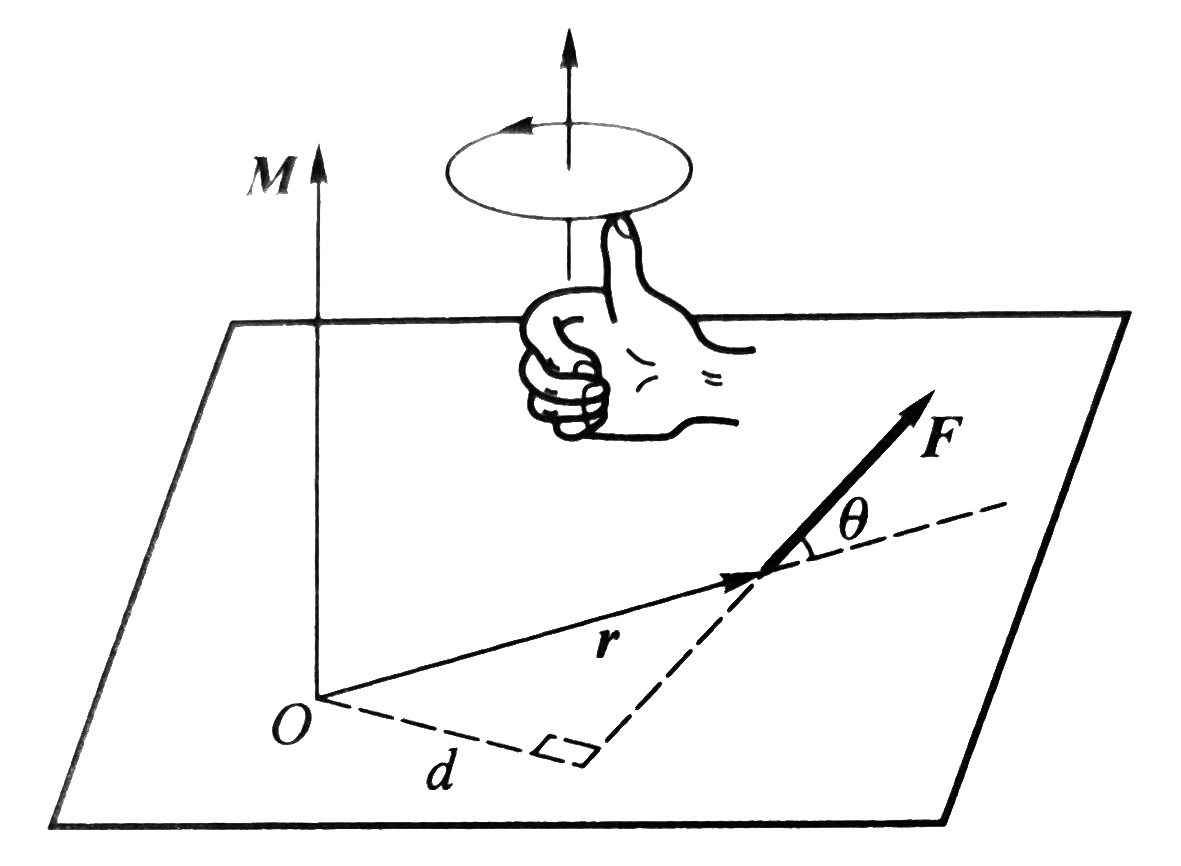
\includegraphics[width=0.45\textwidth]{liju-1}
		\caption{力矩示意图.}
		\end{center}
	\end{figure}

	角动量:一个动量为${\boldsymbol p}$的质点,对于惯性系中某一个参考点$O$的角动量${\boldsymbol L}$(动量矩)定义为:
	\begin{equation*}
		{\boldsymbol L}={\boldsymbol r}\times{\boldsymbol p}={\boldsymbol r}\times m{\boldsymbol v}.
	\end{equation*}

	其大小为:
	\begin{equation*}
		{\boldsymbol L}=rpsin\theta=mrvsin\theta.
	\end{equation*}

	其中$\theta$为${\boldsymbol r}$和${\boldsymbol p}$的夹角,${\boldsymbol L}$的方向由右手螺旋定则确定.
	\begin{figure}[h]
		\begin{center}
		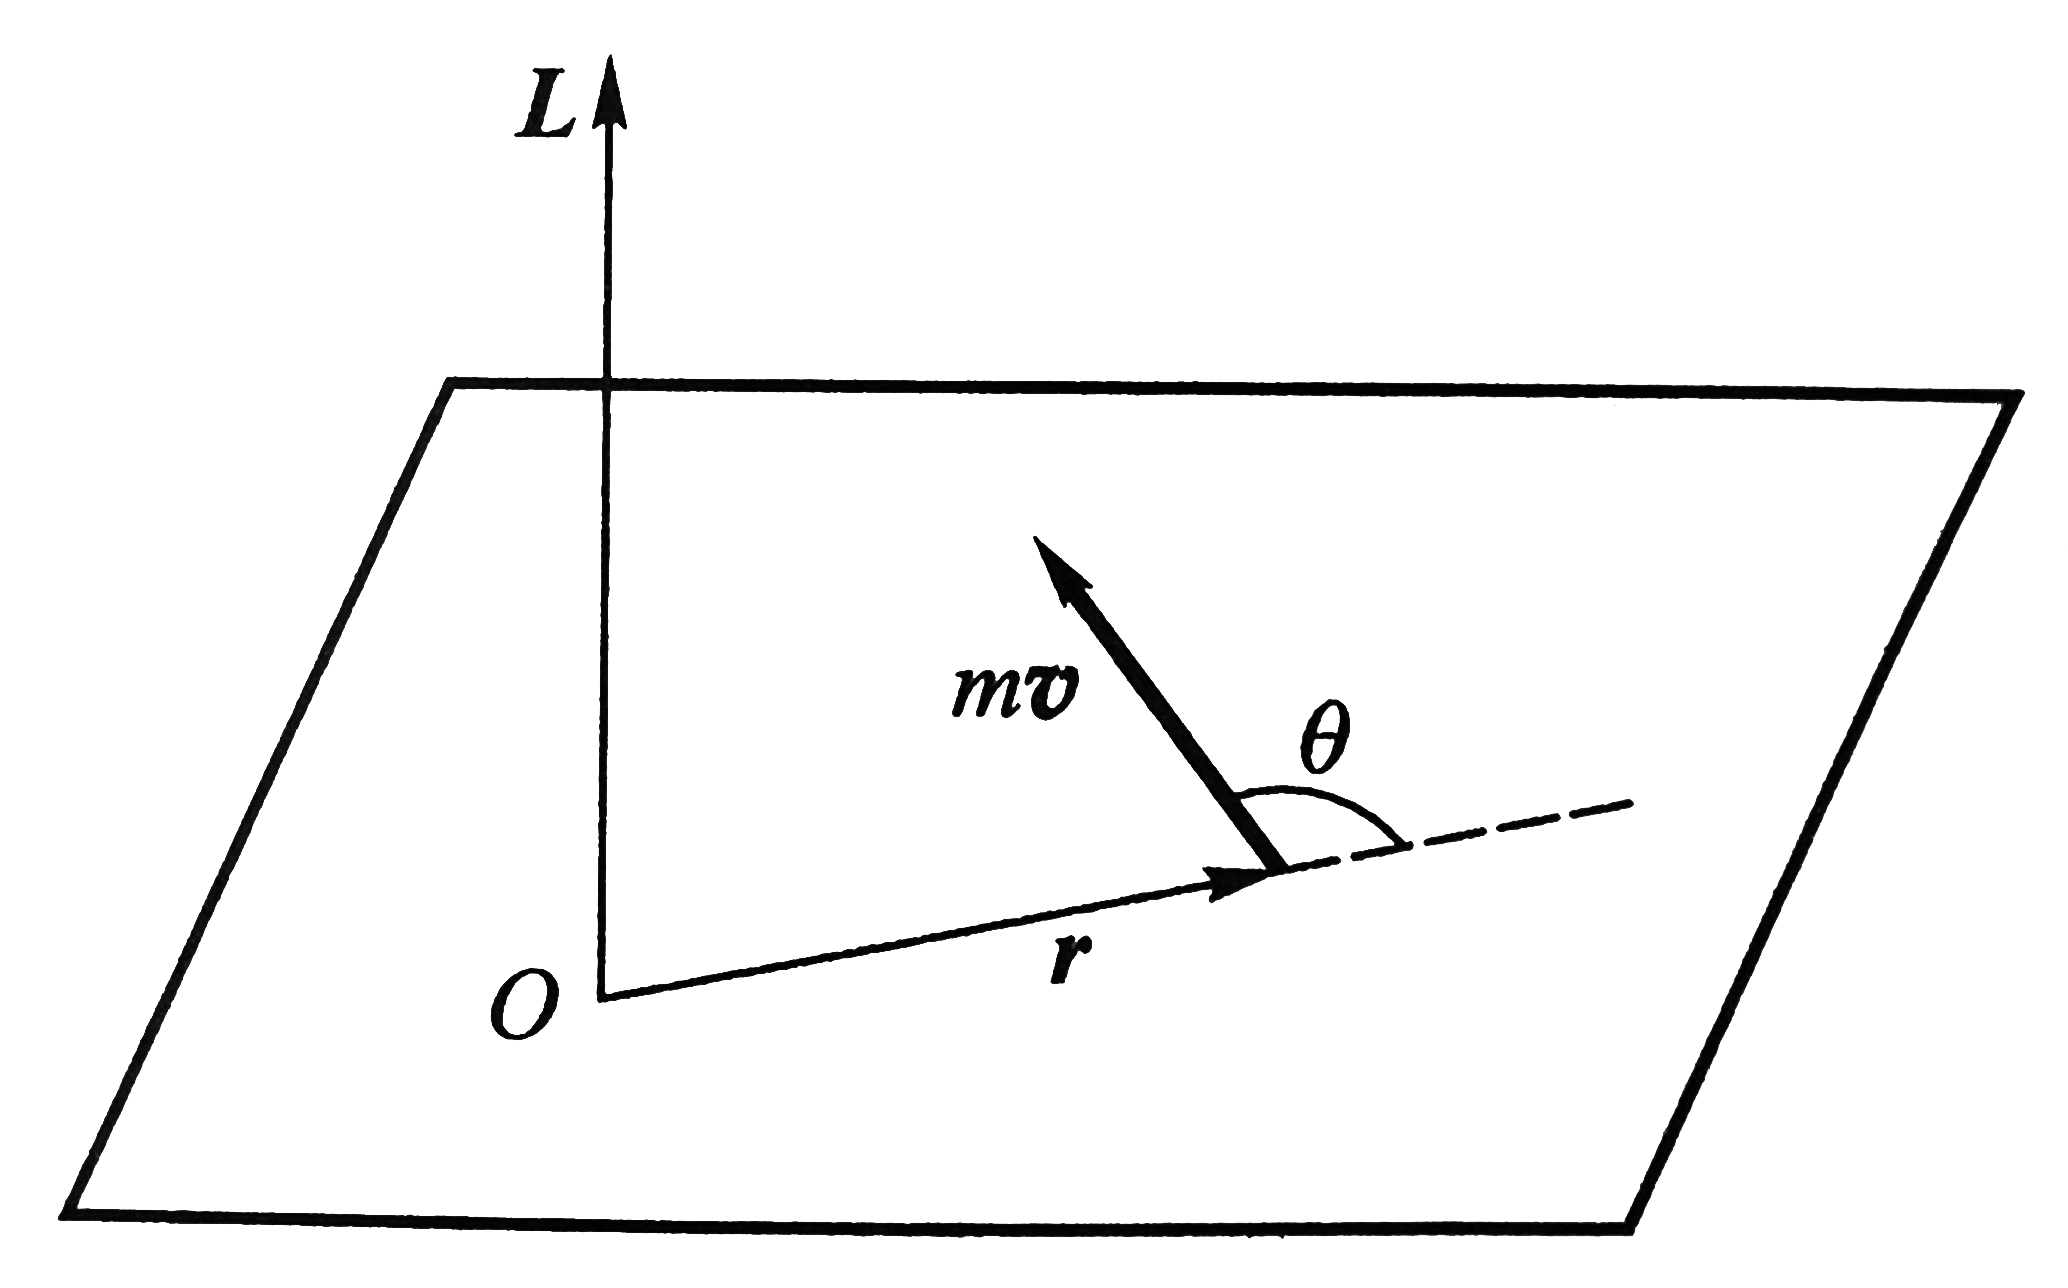
\includegraphics[width=0.45\textwidth]{jiaodongliang-2}
		\caption{角动量示意图.}
		\end{center}
	\end{figure}

	当质点做圆周运动时,质点对圆心的角动量大小为:
	\begin{equation*}
		{\boldsymbol L}=rp=rmv=mr^2\omega.
	\end{equation*}

	质点的角动量定理:质点所受的合外力矩等于它的角动量对时间的变化率,即:
	\begin{equation*}
		{\boldsymbol M}=\frac{d{\boldsymbol F}}{dt}.
	\end{equation*}

	积分可以得到:
	\begin{equation*}
		\int_{t_1}^{t_2}{\boldsymbol M} \,dt={\boldsymbol L}_2-{\boldsymbol L}_1.
	\end{equation*}

	$\int_{t_1}^{t_2}{\boldsymbol M} \,dt$称为合外力矩${\boldsymbol M}$在$t_1$到$t_2$之间的角冲量.即有:质点的角动量的增量等于作用于质点的角冲量,该定理称之为质点的角动量定理.

	质点的角动量守恒定律:若对某一参考点,质点所受的合外力矩为零,则此质点对该参考系的角动量将保持不变,即:
	\begin{equation*}
		{\boldsymbol L}=\text{常矢量}.
	\end{equation*}	

	需要特别注意的是,质点角动量守恒只有两种情况:

	(1)质点所受合外力的匀速直线运动相对于惯性系某参考点角动量守恒;

	(2)质点在有心力的作用下的运动相对于力心的角动量守恒

	$11^{\circ}$相对运动:

	关于位置与速度的相对性,有伽利略位矢变换式和伽利略速度变换式.

	力学相对性原理:在所有相互做匀速直线运动的惯性系中,其力学规律的表达形式都是相同的.
	\subsubsection*{1.2.2例题}



\newpage
%%%%%%%%%%%%%%%%%%%%%%%%%%%%%%%%%%%%%%%%%%%%%%%%%%%%%%%%%%%%%%
%刚体力学
%%%%%%%%%%%%%%%%%%%%%%%%%%%%%%%%%%%%%%%%%%%%%%%%%%%%%%%%%%%%%%
	\section*{$\S$2~~刚体力学}
%-------------------------------------------------------------
%刚体力学
%-------------------------------------------------------------
	\subsection*{刚体力学}
	\subsubsection*{2.1.1基本概念}
	$1^{\circ}$刚体的两类基本运动:平动,绕轴运动.

	$2^{\circ}$描述刚体运动的物理量:
	\begin{equation*}
		\text{角坐标}\theta\text{,}\text{角位移} \Delta\theta\text{,}\text{角速度}{\boldsymbol \omega}\text{,}\text{角加速度} {\boldsymbol\alpha}.
	\end{equation*}

	一般规定,沿逆时针方向的角位移为正.

	关系如下:
	
	角速度的方向由右手螺旋定则决定.
	
	刚体上任一质元$P$的线速度${\boldsymbol v}$与角速度${\boldsymbol \omega}$的关系为:
	\begin{equation*}
		{\boldsymbol v}={\boldsymbol \omega}\times{\boldsymbol r}.
	\end{equation*}
	其中,${\boldsymbol r}$为质元到轴的距离,上述三个物理量相互垂直,大小关系为$v=\omega r$,其中${\boldsymbol \omega}$的方向沿转轴.

	离转轴距离为${\boldsymbol r}$的质元$P$的切向加速度${\boldsymbol a}_t$和法向加速度${\boldsymbol a}_n$与刚体的角速度${\boldsymbol \omega}$和角加速度${\boldsymbol \alpha}$的关系分别为:
	\begin{equation*}
		a_t=\alpha r\text{,}a_n=\frac{v^2}{r}=\omega^2r.
	\end{equation*}

	显然,角加速度${\boldsymbol \alpha}$的方向沿转轴,因此常用标量表示.

	$3^{\circ}$刚体的转动动能定义如下:
	\begin{equation*}
		E_k=\frac{1}{2}J\omega^2.
	\end{equation*}

	$2^{\circ}$转动惯量:
	刚体的转动惯量等于每个质元的质量与这一质元到转轴的距离的平分的乘积的总和,即:
	\begin{equation*}
		\int r^2 \,dm.
	\end{equation*}

	附录给出了形状对称,密度均匀的几种刚体对不同转轴的转动惯量.

	可以看出,刚体的转动惯量与下列因素有关:(1)刚体的质量;(2)转轴的位置;(3)质量分布.

	必须指出,转动惯量是标量,且具有可加性。一个具有复杂形状的刚体,如果可以拆分成若干个简单部分,则整个刚体对某一轴的转动惯量等于各个组成部分对同一轴的转动惯量之和.

	平行轴定理:如果刚体对通过质心轴的转动惯量为$J_C$,那么对此轴平行的任意轴的转动惯量可以表示为
	\begin{equation*}
		J=J_c+md^2.
	\end{equation*}

	其中$m$为刚体的质量,$d$为量平行轴之间的距离.

	$3^{\circ}$转动定律:作用于刚体上的合外力矩等于刚体对转轴的转动惯量与角加速度的乘积,即:
	\begin{equation*}
		{\boldsymbol M}=J{\boldsymbol \alpha}.
	\end{equation*}
	
	显然,力矩是使刚体转动状态改变而产生角加速度的原因.

	值得一提的是,在应用转动定律解题时,基本方法仍然是隔离体法。对于由平动物体和转动物理组成的系统,隔离物体,对平动物体进行受力分析,应用牛顿第二定律;对转动物体进行受力矩分析,应用转动定律.如果方程数不够,可以从线量与角量的关系等方面找到辅助方程.

	$4^{\circ}$力矩的功:定轴转动的刚体在转动$d\theta$角过程中,外力矩所做的功等于外力对转轴的力矩与角位移$d\theta$的乘积.如果刚体在力矩${\boldsymbol M}$的作用下绕固定轴从$\theta^1$转到$\theta^2$,力矩所做的功为:
	\begin{equation*}
		W=\int_{\theta_1}^{\theta_2}{\boldsymbol M} \,d\theta.
	\end{equation*}

	若刚体受到几个外力矩的作用,则${\boldsymbol M}$应是合外力矩,而$W$就是合外力矩做的总功.

	力矩的功率可以表示为:
	\begin{equation*}
		P=\frac{dW}{dt}=M\omega.
	\end{equation*}
	
	也就是说,力矩的功率等于力矩与角速度的乘积.

	$5^{\circ}$刚体的动能定理:合外力矩对定轴转动刚体所做的功等于刚体转动动能的增量,即:
	\begin{equation*}
		W=\frac{1}{2}J\omega_2^2-\frac{1}{2}J\omega_1^2.
	\end{equation*}

	$6^{\circ}$包括刚体的机械能守恒定律:

	刚体的重力势能: 刚体的重力势能和将它的全部质量集中在质心处的一个质点所具有的重力势能相同,即:
	\begin{equation*}
		E_p=mgh_c.
	\end{equation*}

	机械能守恒定律:刚体是质点组且任意两点的距离保持不变,所以刚体的内力之功为零.对包括刚体在内的系统而言,在运动过程中,系统所受外力的功与非保守内力功的总和等于系统机械能的增量,即:
	\begin{equation*}
		W_{\text{外}}+W_{\text{非保内}}=\Delta (E_k+E_p)=\Delta E.
	\end{equation*}
	
	这与质点组功能原理完全相同.但在计算机械能时,要考虑质点的动能、刚体的平动动能和转动动能(定轴转动时只计算转动动能)、弹性势能、质点的重力势能和刚体的重力势能.
	
	对于上述系统,如果外力与非保守内力都不做功或做功的代数和为零,则该系统的机械能守恒,即当$W_{\text{外}}+W_{\text{非保内}}=0$时,有:
	\begin{equation*}
		E_k+E_p=\text{常量}.
	\end{equation*}
	
	若刚体在重力作用下做定轴转动,则刚体的重力势能和刚体的转动动能相互转化,总和不变,即:
	\begin{equation*}
		E=\frac{1}{2}J\omega^2+mgh_c=\text{常量}.
	\end{equation*}

	$7^{\circ}$刚体的角动量定理和角动量守恒定律:
	
	刚体的角动量(动量矩):刚体对某转轴的角动量等于刚体对此转轴的转动惯量与角速度的乘积,即:
	\begin{equation*}
		{\boldsymbol L}=J{\boldsymbol \omega}.
	\end{equation*}

	角冲量(冲量矩):作用在刚体上的冲量矩等于其角动量的增量,即:
	\begin{equation*}
		\int_{t_1}^{t_2}{\boldsymbol M} \,dt=J{\boldsymbol \omega}_2-J{\boldsymbol \omega}_1.
	\end{equation*}

	我们发现,在某些物体运动时,转动惯量会发生变化,但上式依然成立,故上式可以改写为:
	\begin{equation*}
		\int_{t_1}^{t_2}{\boldsymbol M} \,dt=J_2{\boldsymbol \omega}_2-J_1{\boldsymbol \omega}_1.
	\end{equation*}

	角动量守恒定律:当物体所受的合外力矩为零时,物体的角动量保持不变,即:
	\begin{equation*}
		J{\boldsymbol \omega}=\text{常量}.
	\end{equation*}

	角动量守恒定律不仅适用于刚体也适用于绕同一转轴转动的多个刚体的组合.下面分几种情况讨论:

	(1)对定轴转动的单个刚体,$J$一般为定值.当$M=0$时,$J{\boldsymbol \omega}_2=J{\boldsymbol \omega}_1$,则${\boldsymbol \omega}_2={\boldsymbol \omega}_1$,角速度不变,表明刚体做匀角速转动或静止.

	(2)对转动惯量可改变的物体(非刚性物体),由于转动物体通过内力作用改变其对转轴的转动惯量,在此情况下,${\boldsymbol \omega}$会随之改变,这样才能保持角动量不变,故$J$增大,${\boldsymbol \omega}$减小;$J$减小,${\boldsymbol \omega}$增大.

	(3)对由$n$个物体(包括质点)组成的系统,各物体对同一转轴的角动量分别为$J_1{\boldsymbol \omega}_1\text{,}J_2{\boldsymbol \omega}_2\text{,}\dots$,系统的总角动量为$\sum_{i=1}^{n}J_i{\boldsymbol \omega}_i$.只要整个系统受到的合外力矩为零,则系统的总角动量就守恒.
	
	~
	
	在附录中给出了质点动力学与刚体力学规律对照表.
	\subsubsection*{2.2例题}

\newpage
%%%%%%%%%%%%%%%%%%%%%%%%%%%%%%%%%%%%%%%%%%%%%%%%%%%%%%%%%%%%%%
%机械振动	
%%%%%%%%%%%%%%%%%%%%%%%%%%%%%%%%%%%%%%%%%%%%%%%%%%%%%%%%%%%%%%
	\section*{$\S$3~~机械振动}
%-------------------------------------------------------------
%简谐振动
%-------------------------------------------------------------
	\subsection*{3.1简谐振动}
	\subsubsection*{3.1.1基本概念}
	$1^{\circ}$简谐运动的运动方程与运动学判据:
	\begin{equation*}
		x=Acos(\omega t+\varphi ).
	\end{equation*}

	于是有
	\begin{equation*}
		v=-A\omega sin(\omega t+\varphi ).
	\end{equation*}
	\begin{equation*}
		a=-A\omega^2cos(\omega t+\varphi ).
	\end{equation*}

	$2^{\circ}$描写简谐振动的物理量:
	
	(1)振幅:简谐振动物体离开平衡位置最大位移(或最大角位移)的绝对值$A$,称为振幅.

	振幅的大小为:
	\begin{equation*}
		A=\sqrt{x_0^2+\frac{v_0^2}{\omega^2}}.
	\end{equation*}

	(2)周期:物体完成一次全振动所经历的时间叫做振动的周期,用$T$表示.

	周期的值为:
	\begin{equation*}
		T=\frac{2\pi }{\omega}.
	\end{equation*}

	对于弹簧振子,周期为:
	\begin{equation*}
		T=2\pi \sqrt{\frac{m}{k}}.(\omega=\sqrt{\frac{k}{m}})
	\end{equation*}

	对于单摆,周期为:
	\begin{equation*}
		T=2\pi \sqrt{\frac{l}{g}}.(\omega=\sqrt{\frac{g}{l}})
	\end{equation*}

	对于复摆,周期为:
	\begin{equation*}
		T=2\pi \sqrt{\frac{J}{mgl}}.(\omega=\sqrt{\frac{mgl}{J}})
	\end{equation*}

	(3)频率:物体单位时间内所做的完全振动的次数称为频率,记作$v$.

	频率与周期的关系为:
	\begin{equation*}
		v=\frac{1}{T}=\frac{\omega}{2\pi}.
	\end{equation*}

	由于,所以称$\omega$为振动的圆频率(角频率).

	(4)相位:量值$\omega t+\varphi $叫做振动的相位,相位决定简谐振动物体的运动状态.$\varphi$叫做初相位,简称初相,初相的值在一般情况下是:
	\begin{equation*}
		\varphi=arctan\frac{-v_0}{\omega x_0}.
	\end{equation*}

	~

	关于单摆与复摆的内容详见附录.

	$3^{\circ}$简谐振动的矢量表示法:用单位圆与向量表示简谐运动状态的方法叫旋转矢量表示法.
	\begin{figure}[h]
		\begin{center}
			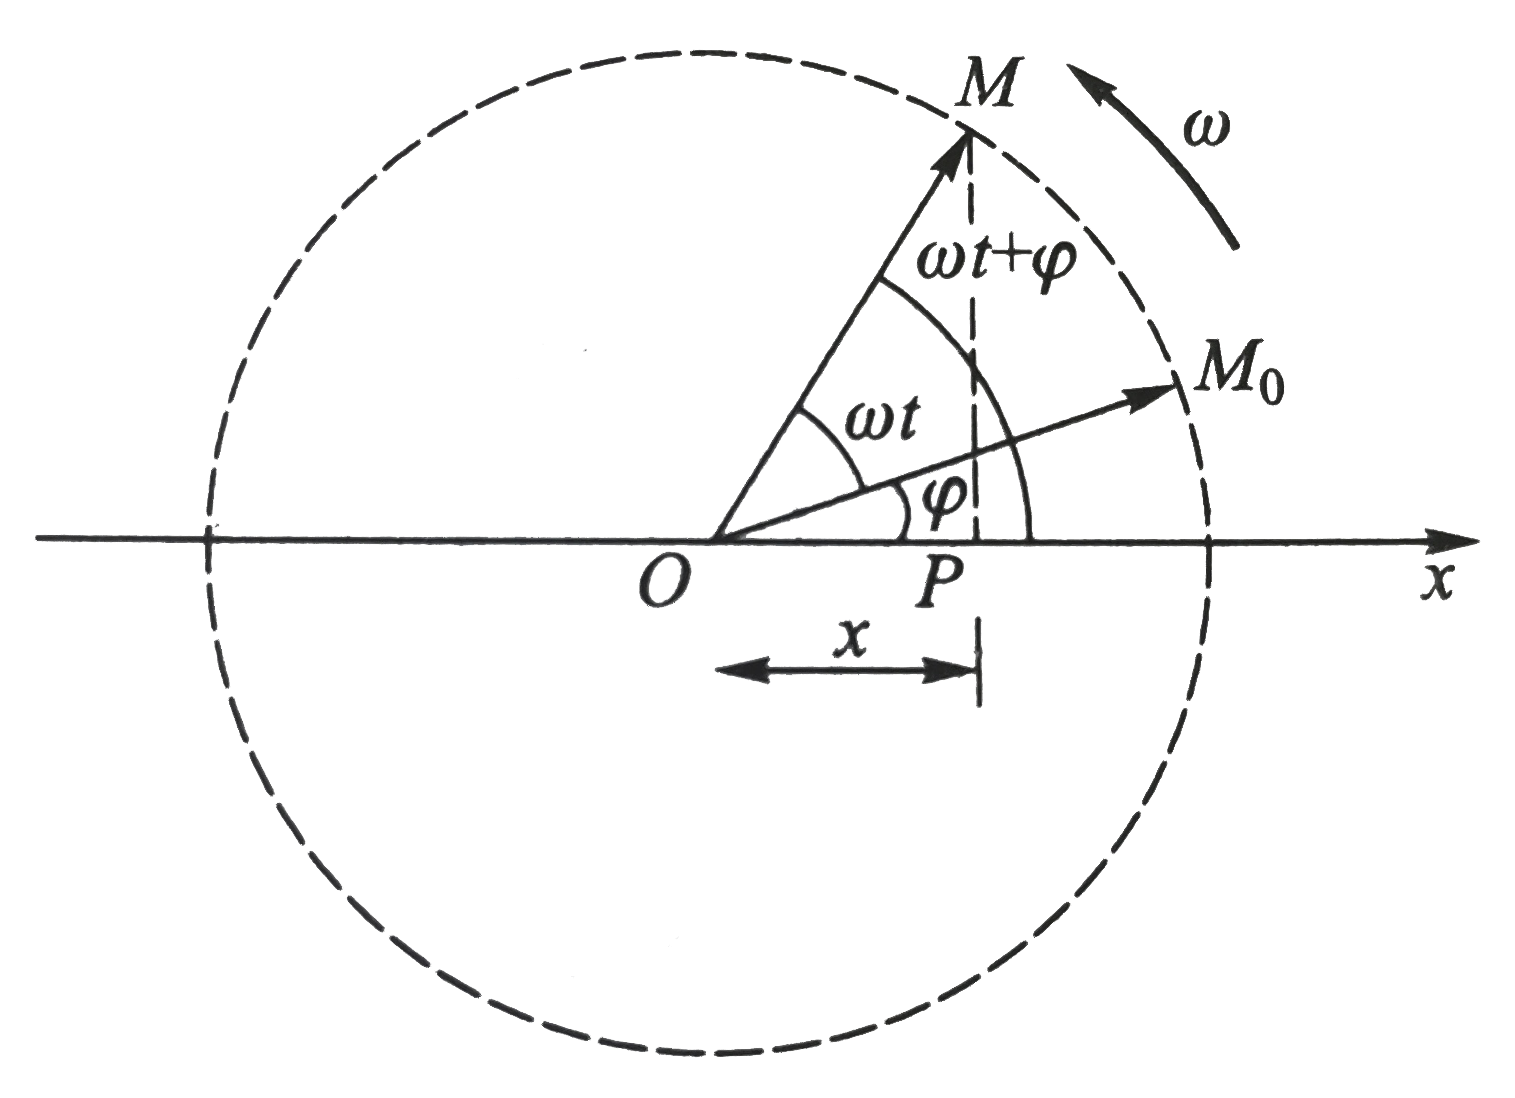
\includegraphics[width=0.45\textwidth]{xuanzhuanshiliang}
			\caption{旋转矢量表示法示意图.}
		\end{center}
	\end{figure}

	由旋转矢量,可以定义简谐运动相位有超前、落后、同相或同步、反相几种状态.

	$4^{\circ}$简谐振动的能量:

	某一时刻弹簧振子的动能和势能为:
	\begin{equation*}
		E_k=\frac{1}{2}m\omega^2A^2sin^2(\omega t+\varphi).
	\end{equation*}
	\begin{equation*}
		E_p=\frac{1}{2}kA^2cos^2(\omega t+\varphi).
	\end{equation*}

	则系统的总能量为:
	\begin{equation*}
		E=\frac{1}{2}kA^2.
	\end{equation*}

	容易得到:弹簧振子的动能在一个周期内的平均值为:
	\begin{equation*}
		\overline{E_k}=\frac{1}{T}\int_{0}^{T}E_k \,dt=\frac{1}{4}kA^2=\frac{1}{2}E.
	\end{equation*}

	显然,势能在一个周期内的平均值也为$\frac{1}{2}E$,这说明弹簧振子的动能和势能在一个周期内的平均值相等且均等于总机械能的一半.这一结论也适用于其他的简谐运动.

	\subsubsection*{3.1.2例题}



%-------------------------------------------------------------
%简谐振动的合成
%-------------------------------------------------------------
	\subsection*{3.2简谐振动的合成}
	\subsubsection*{3.2.1基本概念}
	$1^{\circ}$两个同方向同频率简谐振动的合成:



	$2^{\circ}$两个同方向频率相近简谐振动的合成:

	$3^{\circ}$两个相互垂直同频率简谐振动的合成:

\newpage
%%%%%%%%%%%%%%%%%%%%%%%%%%%%%%%%%%%%%%%%%%%%%%%%%%%%%%%%%%%%%%
%机械波
%%%%%%%%%%%%%%%%%%%%%%%%%%%%%%%%%%%%%%%%%%%%%%%%%%%%%%%%%%%%%%
	\section*{$\S$4~~机械波}
	\subsection*{机械波}
	\subsubsection*{4.1.1基本概念}
	$1^{\circ}$机械波的基本概念

	$2^{\circ}$平面简谐波的波函数

	$3^{\circ}$波的能量

	$4^{\circ}$波的衍射、反射、折射

	$5^{\circ}$波的干涉

	$6^{\circ}$驻波

	$7^{\circ}$多普勒效应

\newpage
%%%%%%%%%%%%%%%%%%%%%%%%%%%%%%%%%%%%%%%%%%%%%%%%%%%%%%%%%%%%%%
%热学	
%%%%%%%%%%%%%%%%%%%%%%%%%%%%%%%%%%%%%%%%%%%%%%%%%%%%%%%%%%%%%%
	\section*{$\S$5~~热学}
	\subsection*{5.1统计物理学}
	\subsubsection*{5.1.1基本概念}
	$1^{\circ}$统计物理学概念

	$2^{\circ}$理想气体的物理量

	$3^{\circ}$麦克斯韦分子速率分布律与玻尔兹曼分布律

	\subsection*{5.2热力学基础}
	\subsubsection*{5.2.1基本概念}
	$1^{\circ}$热力学第一定律:

	系统从一个状态到另一个状态的变化过程称为热力学过程,简称过程.

	准静态过程:系统所经历的没一个中间状态都无限接近于平衡态的过程

	

	$2^{\circ}$热力学第二定律:

	$3^{\circ}$熵增加原理:

\newpage
%%%%%%%%%%%%%%%%%%%%%%%%%%%%%%%%%%%%%%%%%%%%%%%%%%%%%%%%%%%%%%
%波动光学	
%%%%%%%%%%%%%%%%%%%%%%%%%%%%%%%%%%%%%%%%%%%%%%%%%%%%%%%%%%%%%%
	\section*{$\S$6~~波动光学}
	\subsection*{波动光学}
	\subsubsection*{5.2.1基本概念}


\newpage
\section*{$\S$7~~电磁学}
\subsection*{7.1静电场}
\subsubsection*{7.1.1基本概念}
	$1^{\circ}$电荷守恒定律:在一个与外界没有电荷交换的系统内,正负电荷的代数和在任何物理过程中保持不变.
	$2^{\circ}$库仑力:在真空中,两个静止的点电荷之间的相互作用力$F$,与两个电荷的电荷量$q_1$,$q_2$的乘积成正比,与它们之间的距离$r$成反比,力的方向沿两电荷的连线.即:
	\begin{equation*}
		{\boldsymbol F}=\frac{1}{4\pi\xi_0}\frac{q_1q_2}{r^2}{\boldsymbol e}_r.
	\end{equation*}
	式中,${\boldsymbol e}_r$为真空电容率.

\newpage
%%%%%%%%%%%%%%%%%%%%%%%%%%%%%%%%%%%%%%%%%%%%%%%%%%%%%%%%%%%%%%
%参考文献	
%%%%%%%%%%%%%%%%%%%%%%%%%%%%%%%%%%%%%%%%%%%%%%%%%%%%%%%%%%%%%%
	\section*{参考文献}
		[1]杨兵初,李旭光.大学物理学(上册)[M].北京:高等教育出版社.

		[2]杨兵初,李旭光.大学物理学(下册)[M].北京:高等教育出版社.

		[3]马文蔚.物理学(上册)[M].北京:高等教育出版社.

		[4]马文蔚.物理学(下册)[M].北京:高等教育出版社.

\newpage
\section*{附录}
\begin{table}[h]
	\centering
	\begin{tabular}{cc|cc}
	\hline
	\begin{minipage}[b]{0.3\columnwidth}
		\centering
		\raisebox{-.5\height}{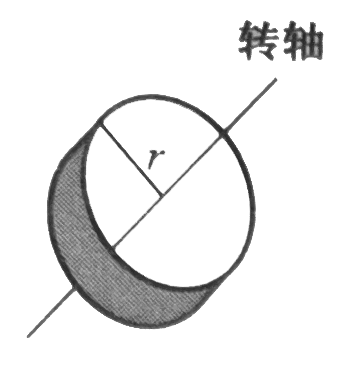
\includegraphics[width=0.4\linewidth]{zhuandongguanliang1}}
	\end{minipage}
	&\tabincell{c}{圆环\\${\boldsymbol J}=mr^2$}
	&\begin{minipage}[b]{0.3\columnwidth}
		\centering
		\raisebox{-.5\height}{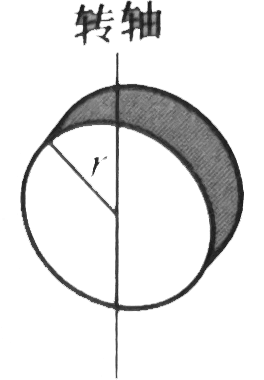
\includegraphics[width=0.3\linewidth]{zhuandongguanliang2}}
	\end{minipage}
	&\tabincell{c}{圆环\\${\boldsymbol J}=\frac{1}{2}mr^2$}
	\\
	\hline
	\begin{minipage}[b]{0.3\columnwidth}
		\centering
		\raisebox{-.5\height}{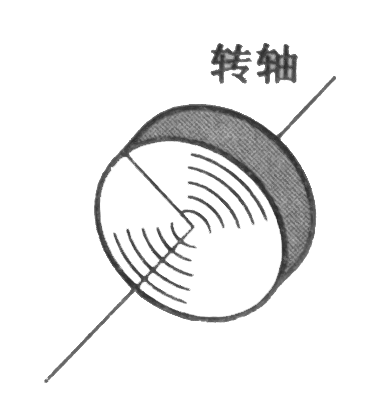
\includegraphics[width=0.4\linewidth]{zhuandongguanliang3}}
	\end{minipage}
	&\tabincell{c}{薄圆盘\\${\boldsymbol J}=\frac{1}{2}mr^2$}
	&\begin{minipage}[b]{0.3\columnwidth}
		\centering
		\raisebox{-.5\height}{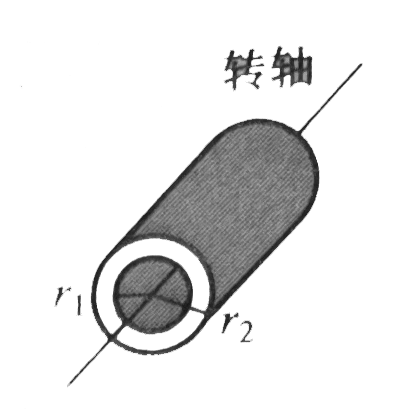
\includegraphics[width=0.4\linewidth]{zhuandongguanliang4}}
	\end{minipage}
	&\tabincell{c}{圆筒\\${\boldsymbol J}=\frac{m}{2}(r_1^2+r_2^2)$}
	\\
	\hline
	\begin{minipage}[b]{0.3\columnwidth}
		\centering
		\raisebox{-.5\height}{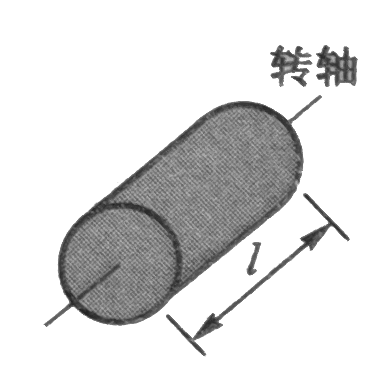
\includegraphics[width=0.4\linewidth]{zhuandongguanliang5}}
	\end{minipage}
	&\tabincell{c}{圆柱体\\${\boldsymbol J}=\frac{1}{2}mr^2$}
	&\begin{minipage}[b]{0.3\columnwidth}
		\centering
		\raisebox{-.5\height}{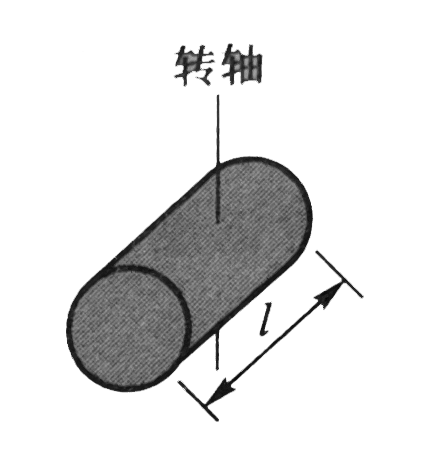
\includegraphics[width=0.4\linewidth]{zhuandongguanliang6}}
	\end{minipage}
	&\tabincell{c}{圆柱体\\${\boldsymbol J}=\frac{1}{4}mr^2+\frac{1}{12}ml^2$}
	\\
	\hline
	\begin{minipage}[b]{0.3\columnwidth}
		\centering
		\raisebox{-.5\height}{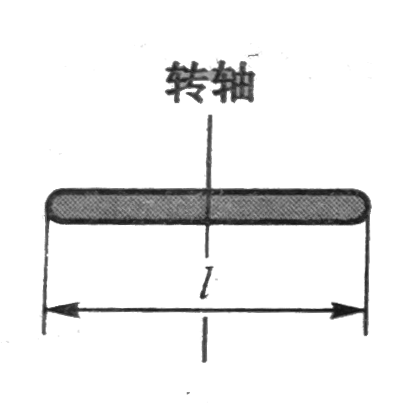
\includegraphics[width=0.4\linewidth]{zhuandongguanliang7}}
	\end{minipage}
	&\tabincell{c}{细棒\\${\boldsymbol J}=\frac{1}{12}ml^2$}
	&\begin{minipage}[b]{0.3\columnwidth}
		\centering
		\raisebox{-.5\height}{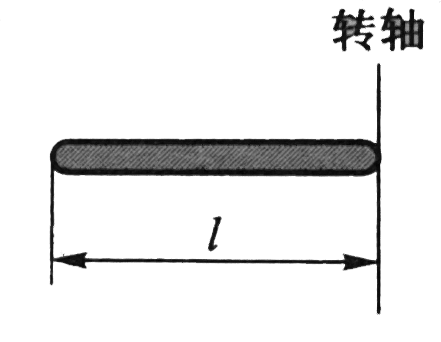
\includegraphics[width=0.4\linewidth]{zhuandongguanliang8}}
	\end{minipage}
	&\tabincell{c}{圆柱体\\${\boldsymbol J}=\frac{1}{3}ml^2$}
	\\
	\hline
	\begin{minipage}[b]{0.3\columnwidth}
		\centering
		\raisebox{-.5\height}{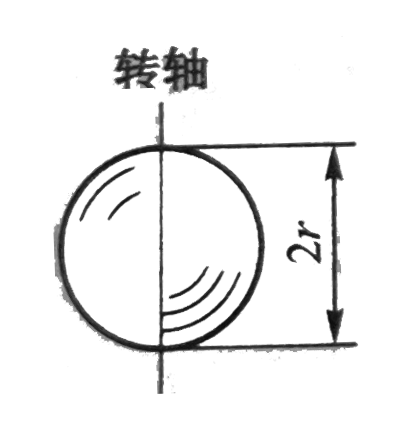
\includegraphics[width=0.4\linewidth]{zhuandongguanliang9}}
	\end{minipage}
	&\tabincell{c}{球体\\${\boldsymbol J}=\frac{2}{5}mr^2$}
	&\begin{minipage}[b]{0.3\columnwidth}
		\centering
		\raisebox{-.5\height}{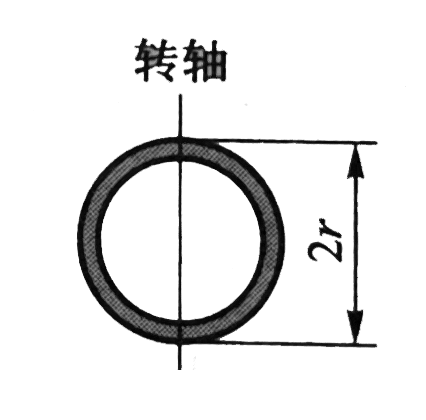
\includegraphics[width=0.4\linewidth]{zhuandongguanliang10}}
	\end{minipage}
	&\tabincell{c}{球壳\\${\boldsymbol J}=\frac{2}{3}mr^2$}\\
	\hline
	\end{tabular}
	\caption{几种规则形状刚体的转动惯量}
	\label{fig-tab1}	
\end{table}
\rule[0pt]{14.3cm}{0.1em}

~

\begin{table*}[htbp]
	\centering
	\begin{tabular}{c|c}
	\hline
	质点 & 刚体\\
	\hline
	力${\boldsymbol F}$,质量$m$&力矩${\boldsymbol M}={\boldsymbol F}\times{\boldsymbol r}$,转动惯量$\int r^2 \,dm.$\\
	牛顿第二定律${\boldsymbol F}=m{\boldsymbol a}$&转动定律${\boldsymbol M}=J{\boldsymbol \alpha}$\\
	动量$m{\boldsymbol v}$,冲量$\int {\boldsymbol F} \,dt$&角动量${\boldsymbol L}=J{\boldsymbol \omega}$,角冲量$\int {\boldsymbol M} \,dt$\\
	动量定理$\int{\boldsymbol F} \,dt=m{\boldsymbol v}_2-m{\boldsymbol v}_1$&角动量定理$\int{\boldsymbol M} \,dt=J{\boldsymbol \omega}_2-J{\boldsymbol \omega}_1$\\
	动量守恒定律$\sum{\boldsymbol F}=0\text{,}\sum m_i{\boldsymbol v}_i=\text{常矢量}$&角动量守恒定律$\sum{\boldsymbol M}=0\text{,}\sum J_i{\boldsymbol \omega}_i=\text{常矢量}$\\
	平动动能$E_k=\frac{1}{2}mv^2$&转动动能$E_k=\frac{1}{2}J\omega^2$\\
	力的功$W=\int{\boldsymbol F} \,d{\boldsymbol r}$&力矩的功$W=\int{\boldsymbol M} \,d\theta$\\
	动能定理$W=\frac{1}{2}mv_2^2-\frac{1}{2}mv_1^2$&动能定理$W=\frac{1}{2}J\omega_2^2-\frac{1}{2}J\omega_1^2$\\
	\hline
	\end{tabular}
	\label{fig-tab1}	
	\caption{质点动力学与刚体力学规律对照表}
\end{table*}

\end{document}
\begin{table}[h]
	\centering
	\begin{tabular}{ | c | l | l | }
	  \hline
	  Items & Advantages & Disadvantages \\ \hline
	  \begin{minipage}[b]{0.3\columnwidth}
		  \centering
		  \raisebox{-.5\height}{\includegraphics[width=\linewidth]{Picture1.png}}
	  \end{minipage}
	  & blabla
	  & blabla
	  \\ \hline
	\end{tabular}
	\caption{Name of this table}
  \end{table}
  
%-------------------------------------------------------------
%普通物理学下
%-------------------------------------------------------------


%%%%%%%%%%%%%%%%%%%%%%%%%%%%%%%%%%%%%%%%%%%%%%%%%%%%%%%%%%%%%%
%%%%%%%%%%%%%%%%%%%%%%%%%%%%%%%%%%%%%%%%%%%%%%%%%%%%%%%%%%%%%%

	%预备代码
	\newpage
	
	\section{问题背景与重述}
		问题背景与重述
		
	\section{模型假设}
		模型假设
	\section{符号说明}
		\begin{longtable}{p{8cm}<{\centering}p{7.5cm}}
			\toprule  %添加表格头部粗线
			符号& 意义\\
			\midrule  %添加表格中横线
			Steve Jobs& 001\\
			Bill Gates& 002\\
			\bottomrule %添加表格底部粗线
		\end{longtable}
		
	\section{问题分析}
		问题分析
		\subsection{问题一分析}
		\subsection{问题二分析}
		\subsection{问题三分析}
		
	\section{模型建立与求解}
		\subsection{问题一模型的建立}
		\subsection{问题一模型的求解}
		
	\section{模型评价与改进}
		模型评价与改进
		
	\section{参考文献}
		参考文献
		
	\newpage
	\section{附录}

